\chapter{Practical Considerations}

In~\pref{cha:solution-approach}, we discussed the theoretical basis for shape-constraint P-splines and their ability to incorporate a priori domain knowledge by choice of the constraint term described by the mapping matrix $\vec{D}_c$ and the weighting matrix $\vec{V}_c$. We will now consider the practical application of these, as well as their limits in terms of data fitting and constraint fidelity. 

It is important to notice that the addition of the constraint term in~\pref{eq:OF-SCP-Final} further reduces the effective degree of freedom of the model, similar as for P-splines, resulting in a less flexible model. We therefore expect that the measured metric on the training data will be worse compared to a pure B-spline fit. Nevertheless, the metric of interest is the measured error on the validation data, i.e. the held out data that the model has not seen before. Supposing that the a priori domain knowledge reflects the true, underlying function behavior, we expect the measured error on the validation data to be lower than or equal to the error given by an optimal P-spline fit. Here, optimality is based on the optimal smoothing parameter $\lambda$ given by generalized cross-validation, see Section~\ref{subsubsec:Cross-validation}. This can be seen by recognizing the equivalence of the objective functions for P-splines, see~\pref{eq:P-spline-final-OF}, and shape-constraint P-splines, see~\pref{eq:OF-SCP-Final}, when the underlying B-spline fit does not violate the user-defined constraint, i.e. all $v_j=0$. This feature is one of the limits of shape-constraint P-splines, i.e. we cannot influence the model using this approach if no constraint violations are present. On the other hand, if the a priori domain knowledge reflects the underlying function, we can expect a far better generalization capability of the model compared to the B-spline fits, especially in situations of noisy or sparse data.

In this chapter, we are going to discuss the practical incorporation of a priori domain knowledge based on the example of peak behavior. We will evaluate the performance of shape-constraint P-splines using noisy, see~\pref{sec:peak-behav-noisy}, and sparse data, see~\pref{sec:peak-behav-sparse}, and compare it to B-splines and P-splines. Further, we will discuss the effect of the constraint parameter $\lambda_c$, see~\pref{sec:lambda_c_sec}.

%%%%%%%%%%%%%%%%%%%%%%%%%%%%%%%%%%%%%%%%%%%%%%%%%%%%%%%%%%%%%%%%%%%%%%%%%%%%%%%%%%%%%%%%%%%%%%%%%%%%%%%%%%%%%%%%%%%%%%%%%%%%%%%%%
\section{Peak Constraint in Practice} \label{sec:peak-behav-noisy}

We will now use shape-constraint P-splines and the a priori domain knowledge of peak behavior to fit the data $\mathcal{D} = \{(x^{(i)}, y^{(i)}), \ i=1,2,\dots,n\}$. The data is artificially generated by random sampling of $n=200$ points $x^{(i)}$ of the function $f$, i.e.

\begin{align} \label{eq:test-func-peak}
	y^{(i)} = f(x^{(i)}) + \epsilon^{(i)} = \exp\left(-\frac{(x^{(i)} - 0.35)^2}{0.1} \right) + \epsilon^{(i)} \quad \text{for} \ x^{(i)} \in [0.1,0.8],
\end{align}
%
with $\epsilon^{(i)}$ being Gaussian noise with mean $\mu = 0$ and variance $\sigma^2 = 0.01$. We randomly split the data in a training set $\mathcal{D}_t$ with 150 samples and a validation set $\mathcal{D}_v$ with 50 samples. At first, we use $d=45$ B-spline basis functions of order $l=3$ to fit a B-spline to the training data $\mathcal{D}_t$. Then, we fit a P-spline using the same number of basis functions $d$ and order $l$ with an optimal smoothness parameter $\lambda_{opt} = 7.74$ chosen by generalized cross-validation. Finally, we enforce the peak behavior by using a shape-constraint P-spline using the same number of basis functions $d$ and order $l$ as well as the optimal smoothness parameter $\lambda_{opt}=7.74$ and the constraint parameter $\lambda_c=6000$ reflecting high trust in the a priori domain knowledge. The various fits are evaluated on the validation data $D_v$ and shown in~\pref{fig:test-func-peak-fit}. The mean squared errors on the validation data, as well as on the true, underlying function in~\pref{eq:test-func-peak}, are given~\pref{tab:test-func-peak-mses}.


\begin{figure}[H]
	\centering
	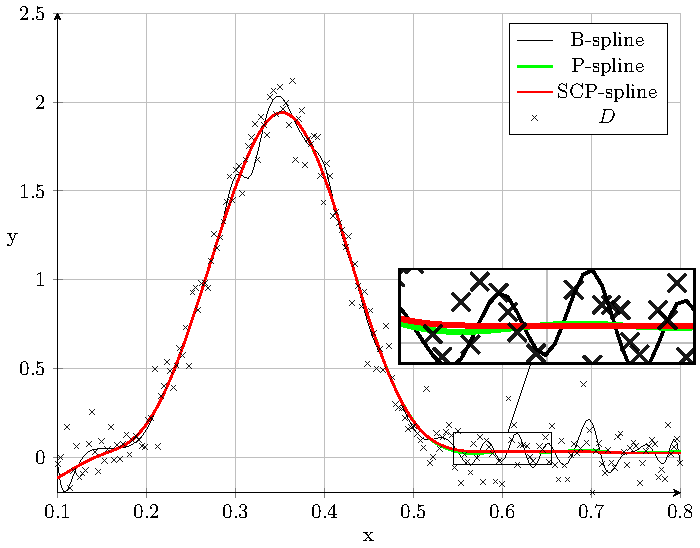
\includegraphics{graphics/pgfplots/cha4/exp-peak.pdf}
	\caption{B-spline, P-spline and SCP-spline fit for the data $\mathcal{D}$.}
	\label{fig:test-func-peak-fit}
\end{figure}
%
The B-spline, as black curve in~\pref{fig:test-func-peak-fit}, captures the basic shape of the true function, but the flexibility of the B-spline, due to the high number of B-splines, leads to a wiggly estimate especially for the almost constant part. This violates the peak behavior of the true function, i.e. being non-increasing after the peak value. For the P-spline (green), this problem relaxes due to the smoothing aspect of the penalty term but does not vanish, as seen in the magnified part in~\pref{fig:test-func-peak-fit}. Note that the additional smoothness penalty given by the P-spline already fits the data almost perfectly. The SCP-spline estimate adjusts only the parts of the P-spline, which violate the constraint. It may be seen as "fine-tuning" of the fit using the a priori domain knowledge. Hence, it is the best solution here as it is nearly constant for the necessary parts of the function in~\pref{eq:test-func-peak}.  

\begin{table}[H]
	\begin{center}
		\pgfplotstabletypeset[
		col sep=comma,
		columns/Model/.style={string type},
		columns/MSEVal/.style={column name={$\text{MSE}_{\mathcal{D}_v}$}},
		columns/MSEValTrueFunction/.style={column name={$\text{MSE}_{\mathcal{D}_{v,true}}$}},
		every head row/.style={before row=\toprule[1pt] \toprule,after row=\midrule[2pt]},
		every last row/.style={after row=\bottomrule \bottomrule},
		every nth row={1}{before row=\midrule},
		]{graphics/data/cha4/peak_example/mse.csv}
	\end{center}
	\caption{Mean squared errors on the validation set $\mathcal{D}_v$.}
	\label{tab:test-func-peak-mses}
\end{table}
%
The mean square errors on the noisy validation data $\mathcal{D}_v$ in~\pref{tab:test-func-peak-mses} for P-spline and SCP-spline are almost identical and do not show a favorable model. Comparing the various models with the true, underlying function, see $\text{MSE}_{D_{v,true}}$ in~\pref{tab:test-func-peak-mses}, leads to the assessment that the SCP-spline is the more accurate model with regards to the true function behavior. This coincides with the graphs in~\pref{fig:test-func-peak-fit}. Hence, the incorporation of a priori domain knowledge via shape-constraints improves the generalization capability measured by the mean squared error on the true function values in our example. 
%%%%%%%%%%%%%%%%%%%%%%%%%%%%%%%%%%%%%%%%%%%%%%%%%%%%%%%%%%%%%%%%%%%%%%%%%%%%%%%%%%%%%%%%%%%%%%%%%%%%%%%%%%%%%%%%%%%%%%%%%%%%%%%%%

\section{Peak Constraint and Sparse Data} \label{sec:peak-behav-sparse}

We will now examine the behavior of B-, P- and SCP-splines for sparse data, i.e. little data and unevenly distributed, sampled from the function in~\pref{eq:test-func-peak}. The data set $D$ now contains 70 data points distributed in a way that there is little data in the peak region, i.e. for $x \in [0.2, 0.5]$ we have only 10 data points. We perform an random train-validation split of the data in $\mathcal{D}$, i.e. the training data $\mathcal{D}_t$ consists of 52 points and the validation data $\mathcal{D}_v$ consists of 18 points. We follow the same approach as above, i.e. fit a B-spline, perform generalized cross-validation to fit the optimal P-spline and finally apply the shape-constraint to enforce peak behavior. The small data set indicates that a different, not equidistant knot placement may be helpful. Hence, we carry out 2 experiments, one with equidistant knot placement and the other with quantile-based knot placement, see Section~\ref{subsec:b-splines}. We chose to use $d=25$ B-spline basis functions of order $l=3$. The optimal smoothness parameter was given as $\lambda_{opt} = 0.00657$ for the equidistant fit and $\lambda_{opt} = 0.00215$ for the quantile-based fit. The constraint parameter $\lambda_c$ was set to $\lambda_c=1000$ for both fits, reflecting high trust in the a priori domain knowledge. The resulting fits are shown in~\pref{fig:sparse-example-equidistant} and~\pref{fig:sparse-example-quantile}.


\begin{figure}[H]
	\centering
	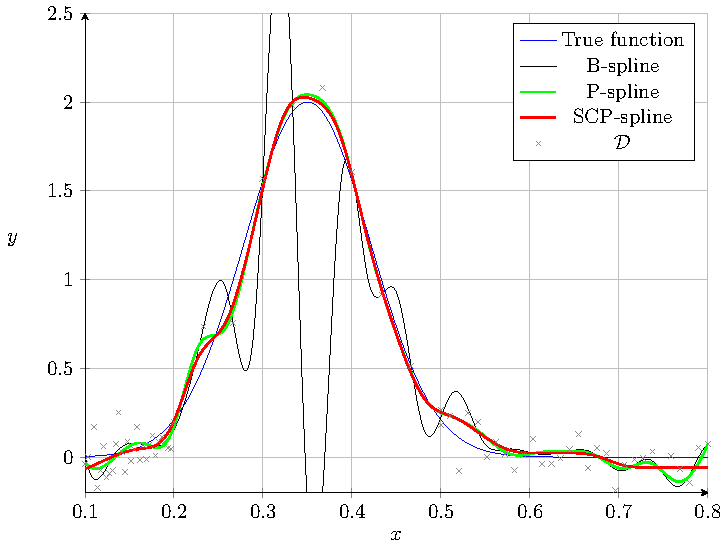
\includegraphics{graphics/pgfplots/cha4/exp-sparse-equidistant.pdf}
	\caption{Equidistant B-spline, P-spline and SCP-spline fit for sparse data $\mathcal{D}$.}
	\label{fig:sparse-example-equidistant}
\end{figure}

The B-spline (black) in~\pref{fig:sparse-example-equidistant} shows the problem of equidistant knot placement in sparse data situations. The estimate becomes very wiggly, similar to polynomial fits using a high degree. Nevertheless, utilizing the regularization through the additional smoothness penalty in P-splines, the estimate (green) becomes smoother and reflects the true function quite well. The shape-constraint P-spline (red) further improves the quality of the fit, as seen in~\pref{tab:sparse-example-equidistant}. 

\begin{table}[H]
	\begin{center}
		\pgfplotstabletypeset[
		col sep=comma,
		columns/Model/.style={string type},
		columns/MSEVal/.style={column name={$\text{MSE}_{\mathcal{D}_v}$}},
		columns/MSEValTrueFunction/.style={column name={$\text{MSE}_{\mathcal{D}_{v,true}}$}},
		every head row/.style={before row=\toprule[1pt] \toprule,after row=\midrule[2pt]},
		every last row/.style={after row=\bottomrule \bottomrule},
		every nth row={1}{before row=\midrule},
		]{graphics/data/cha4/sparse_example/mse-e.csv}
	\end{center}
	\caption{Mean squared errors on the validation set $\mathcal{D}_v$ for equidistant knot placement.}
	\label{tab:sparse-example-equidistant}
\end{table}


\begin{figure}[H]
	\centering
	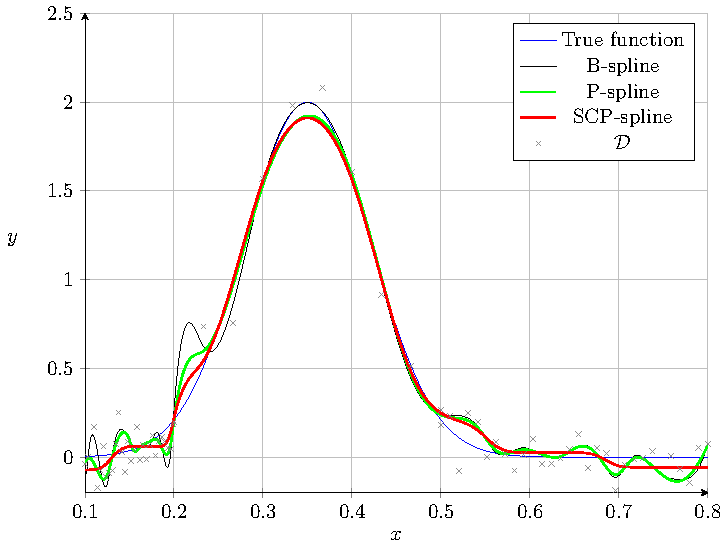
\includegraphics{graphics/pgfplots/cha4/exp-sparse-quantile.pdf}
	\caption{Quantile-based B-spline, P-spline and SCP-spline fit for sparse data $\mathcal{D}$.}
	\label{fig:sparse-example-quantile}
\end{figure}

The quantile-based B-spline (green) in~\pref{fig:sparse-example-quantile} shows some interesting features. At first, it fits the peak surprisingly well despite the small sample size in this area. This is due to the inherent smoothing aspect of quantile-based knot placement in regions of small sample size. Further, we see the flexibility of the B-spline in the regions with more data, i.e. $x\in[0.1,0.2]$ and $x \in [0.5,0.8]$, where it clearly fits the noise part instead of the true function. Hence, quantile-based knot placement may lead to partial overfitting, i.e. overfitting of the estimate only on a part of the input space. Using a P-spline (green) does not relax this problem as the estimates (back and green) overlap almost everywhere. This may be caused by the inability of finding an optimal smoothing parameter value when the distribution of basis functions is not equidistant. Nevertheless, including additional regularization through the shape-constraint leads to an estimate which is smooth, follows the a priori domain knowledge and generalizes better, seen by the comparison of the $\text{MSE}_{D_v}$ and $\text{MSE}_{D_{v, true}}$ in~\pref{tab:sparse-example-quantile}.


\begin{table}[H]
	\begin{center}
		\pgfplotstabletypeset[
		col sep=comma,
		columns/Model/.style={string type},
		columns/MSEVal/.style={column name={$\text{MSE}_{\mathcal{D}_v}$}},
		columns/MSEValTrueFunction/.style={column name={$\text{MSE}_{\mathcal{D}_{v,true}}$}},
		every head row/.style={before row=\toprule[1pt] \toprule,after row=\midrule[2pt]},
		every last row/.style={after row=\bottomrule \bottomrule},
		every nth row={1}{before row=\midrule},
		]{graphics/data/cha4/sparse_example/mse-q.csv}
	\end{center}
	\caption{Mean squared errors on the validation set $\mathcal{D}_v$ for quantile-based knot placement.}
	\label{tab:sparse-example-quantile}
\end{table}


%%%%%%%%%%%%%%%%%%%%%%%%%%%%%%%%%%%%%%%%%%%%%%%%%%%%%%%%%%%%%%%%%%%%%%%%%%%%%%%%%%%%%%%%%%%%%%%%%%%%%%%%%%%%%%%%%%%%%%%%%%%%%%%%%

\section{The Effect of the Constraint Parameter $\lambda_c$} \label{sec:lambda_c_sec}

We will now discuss the effect of the constraint parameter $\lambda_c$. As noted in~\pref{sec:peak-behav-noisy}, the shape-constraint acts as "fine-tuneing" of the estimate according to the a priori domain knowledge, i.e. it only changes the estimate at places where it violates the user-defined shape constraint. We use the constraint parameter $\lambda_c$ as measure of the trust in the a priori domain knowledge, such that high trust is reflected by high values of $\lambda_c$. To show this in practice, we use the data $\mathcal{D}$ given in~\pref{sec:peak-behav-noisy} and fit shape-constraint P-splines using various values of a priori domain knowledge trust reflected by $\lambda_c$. The results are show in~\pref{fig:example-lambdas}. Since most constraint violations are present for larger $x > 0.55$, we focus on this part of the plot. 

\begin{figure}[H]
	\centering
	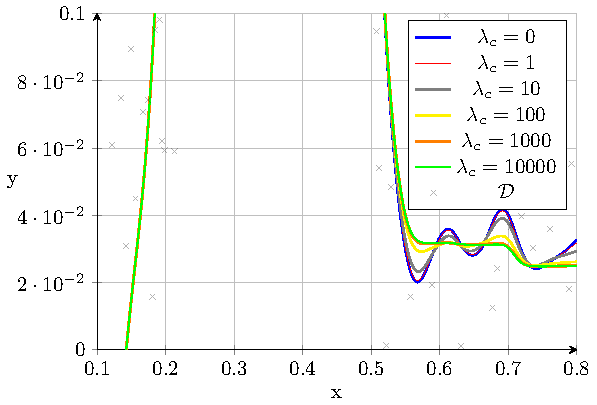
\includegraphics{graphics/pgfplots/cha4/exp-lambdas.pdf}
	\caption{SCP-splines for different $\lambda_c$ for data $\mathcal{D}$.}
	\label{fig:example-lambdas}
\end{figure}	

In~\pref{fig:example-lambdas}, we clearly see that with increasing $\lambda_c$ we enforce the a priori domain knowledge. For small $\lambda_c \le 10$, the estimates (blue, red and gray) violate the constraint qualitatively quite strong. Medium values of $\lambda_c = 100$ already produce an estimate (yellow) that follows the constraint far better, but not optimally. High values of $\lambda_c \ge 1000$ enforce the a priori domain knowledge, as seen by the orange and the green estimate. Nevertheless, quantitatively small violations of the a priori domain knowledge are possible even for this values of the constraint parameters. 


\begin{comment}
\section{Something}
In this chapter we use the theory discussed in Chapter \pref{cha:fundamentals} to estimate uni- and bivariate  functions using data and a priori domain knowledge. An overview of the different problems considered in this chapter is given in Table \pref{tab:problem_overview}. 

\begin{table}[H]
	\centering
	\begin{tabular}{|l|l|l|l|}
		\hline
		\textbf{Univariate}   & \textbf{Section} & \textbf{Bivariate}         & \textbf{Section} \\ \hline \toprule
		B-splines             &                & Tensor-product B-splines   &               \\ \hline
		P-splines             &                & Tensor-product P-splines   &              \\ \hline
		SCP-splines           & 			   & Tensor-product SCP-splines &     \\ \hline \bottomrule
	\end{tabular}
	\caption{Problem overview.}
	\label{tab:problem_overview}
\end{table}
%
First, we are using B-splines, see Section~\pref{subsec:b-splines}, for the estimation of the unknown function $y = f(x)$, i.e. we solve the optimization problem

\begin{align} \label{eq:OF-B-splines}
	\arg \min_{\vec{\beta}} Q_1(\vec{y}, \vec{\beta}) = \lVert \vec{y} - \vec{X} \vec{\beta} \rVert,
\end{align}
%
using the B-spline or tensor-product B-spline basis matrix $\vec{X}$. Next, we use the concept of P-splines, see Section~\pref{subsec:p-splines}, to estimate smooth functions, i.e. we solve the optimization problem

\begin{align} \label{eq:OF-P-splines}
	\arg \min_{\vec{\beta}} Q_2(\vec{y}, \vec{\beta}; \lambda) = \lVert \vec{y} - \vec{X} \vec{\beta} \rVert + \lambda \cdot \text{pen}(\vec{\beta}),
\end{align}
%
where $\text{pen}(\vec{\beta})$ specifies a smoothness penalty term. Finally, we are going to incorporate a priori domain knowledge into the fitting process using shape-constrained P-splines (SCP-splines), i.e. we solve the optimization problem
\begin{align} \label{eq:OF-SCP-splines}
	\arg \min_{\vec{\beta}} Q_3(\vec{y}, \vec{\beta}; \lambda, \lambda_c) = \lVert \vec{y} - \vec{X} \vec{\beta} \rVert + \lambda \cdot \text{pen}(\vec{\beta}) + \lambda_c \cdot \text{con}(\vec{\beta}),
\end{align}
%
where $\text{pen}(\vec{\beta})$ is again a smoothness penalty term and $\text{con}({\vec{\beta}})$ specifies the user-defined shape-constraint to incorporate a priori domain knowledge with, see \cite{hofner2011monotonicity} and \cite{bollaerts2006simple}. Various types a priori domain knowledge can be incorporated using the constraints listed in~\pref{tab:constraint_overview}.



The focus of this chapter is the definition and use of shape-constraint P-splines, which are characterize by their parameters $\vec{\beta}$ given by solving the optimization problem~\pref{eq:OF-SCP-splines}.

\end{comment}
